% !TEX root = ../Thesis.tex
\begin{document}
\documentclass[Thesis.tex]{subfiles}
\chapter{Results}
\label{ch:results}

Vielleicht sollte das Kapitel eher challenges and solutions heißen. Es sind ja nicht nur results, sondern auch immer die Problemstellungen beschrieben.

\section{Duplicate Detection}

%Exploring our dataset we realized that we had to deal with two duplication
%problems. The first being that several letters were contained more
%than once in our dataset. The second, more challenging problem was
%that for several patients letters of different time points with somewhat
%different content were present. To ensure we would not distort
%our results, because of duplicates present in our test set, we tried
%to identify all duplicates of the two kinds. On first glance at least
%the first problem seems easy. Finding exact duplicates is not a challenging
%task. However, as the letters were made anonymous separately, they
%are not exact copies of each other. Names and other personal information
%were eradicated from the word documents by hand, so extra whitespaces
%and similar subtle differences were introduced. For a subset of 150
%of the letters we manually searched for the duplicates. However, this
%work is tedious, error-prone and does not scale to bigger datasets.
%To semi-automatically find the true duplicates and the follow-up letters
%we used two approaches.
%
%The first method searches two letters for their longest common subsequence
%of characters. If this longest common subsequence exceeds a threshold
%relative to the longer document (e.g. 3 \% of the length of the longer
%document), then the two letters are marked as possibly related. In
%the second approach we use the bag of words representations of the
%documents and their cosine distance in the vector space as an indicator.
%If the distance between two vectors is lower than a threshold (e.g.
%0.2), they are also marked as possibly related.
%
%We start in both methods with high thresholds, manually check the results
%and successively lower them until the false positive rate becomes
%too high. With this procedure we were able to quickly find all the
%duplicate pairs we already found manually before. Additionally we
%found two follow-up pairs among the 150 that we did not identify with
%the manual procedure. The bag of words approach is somewhat more reliable
%and identified almost all the duplicates, before including false positives.
%However, we did not find two other duplicates pairs, that
%the string matching procedure quickly identified. So it seems worth
%the effort to use both methods.
%
%Later we found one more follow-up pair by chance. However, these two
%letters are radically different in content and so this event does
%not undermine our confidence, that we were able to find a sufficient
%portion of the duplicate pairs to not distort our test results. (Will ich diesen letzten Absatz überhaupt drin haben?)


\section{Paragraph Extraction}



\section{Paragraph Classification}
In our sample dataset, we can automate paragraph extraction as shown above. We can also semi-automatically detect for which paragraphs the procedure produces incorrect results. This approach works well only because the documents in our dataset generally adhere to a rough structure. For datasets from other clinics constructing a rule based extraction procedure is not only time consuming, it might not be possible at all. We therefore test an approach to classification of extracted paragraphs into the respective categories - greeting, diagnosis and anamnesis. Our findings show that surprisingly this is not a hard problem. On unseen datasets it might therefore be possible to split text into unlabeled paragraphs with a basic rule based approach. One can possibly define a new paragraph to begin after a blank line and automatically label the resulting paragraphs with a predefined category. This way one would be able to hide or show specific information on demand even on datasets from other clinics.

We approach the problem again from a vector space based view-point. We first compute the vector representation for every paragraph with different text embedding methods. Then logistic regression is trained on a training portion of the dataset and the performance evaluated on a testing portion. We use leave-one-out cross-validation to obtain a good estimate of the performance even on our limited dataset.

As vector embedding methods we tested the standard bag of words, tf-idf and paragraph vector models. We also used LSA and LDA to get more condensed feature vector representations based on the tf-idf vector space. Results of our evaluation can be found in table \ref{table:para_class_acc}   . Several things are noteworthy about the results. First it is surprisingly easy in general to use a small number of training paragraphs (less than 300 per category) to predict its label with very high accuracy. Second all methods are indeed outperformed by the more recent paragraph vector approach. However, the paragraph vector performance comes with the cost of needing to tune many hyperparameters, whose influence is not intuitively clear. Third LSA performance is always smaller or equal to tf-idf performance. As the tf-idf vector space has several thousand dimensions, but we only have several hundred texts, all these texts must fall into a linear subspace with dimension no greater than the number of texts. We assume the dimension is even substantially smaller, as LSA vectors produce the same results in classification accuracy when reducing the number of dimensions until 21. Reducing dimensionality further diminishes accuracy. 

To gain a more intuitive understanding of the performance of these approaches we use PCA to get a 2D approximation of the vectors of the extracted paragraphs. In figure \ref{fig:pv_tf_pca} one can compare the 2D PCA projections of the tf-idf and the paragraph vector models. While it is obvious that both methods can produce good results even just using a linear classifier, it is also easy to see that the paragraph vectors are easier separable (although not linearly separable in the 2D projection). We conclude that paragraph vector is the best suited method for this classification task and surprisingly performs well even with very limited training data, a finding not documented in the literature.
\begin{table}
\begin{tabular}{|c|c|c|c|c|c|}
	\hline 
	Embedding Method & BOW & TF-IDF & LSA & LDA  & Para2Vec\tabularnewline
	\hline 
	\hline 
	Classification Accuracy & 0.995 & 0.997 & 0.997 & 0.992 & \underline{1.0}\tabularnewline
	\hline 
\end{tabular}
	\caption{Mean classification accuracy of logistic regression with leave-one-out crossvalidation by vector embedding methods.}
	\label{table:para_class_acc}
\end{table}

\begin{figure}
	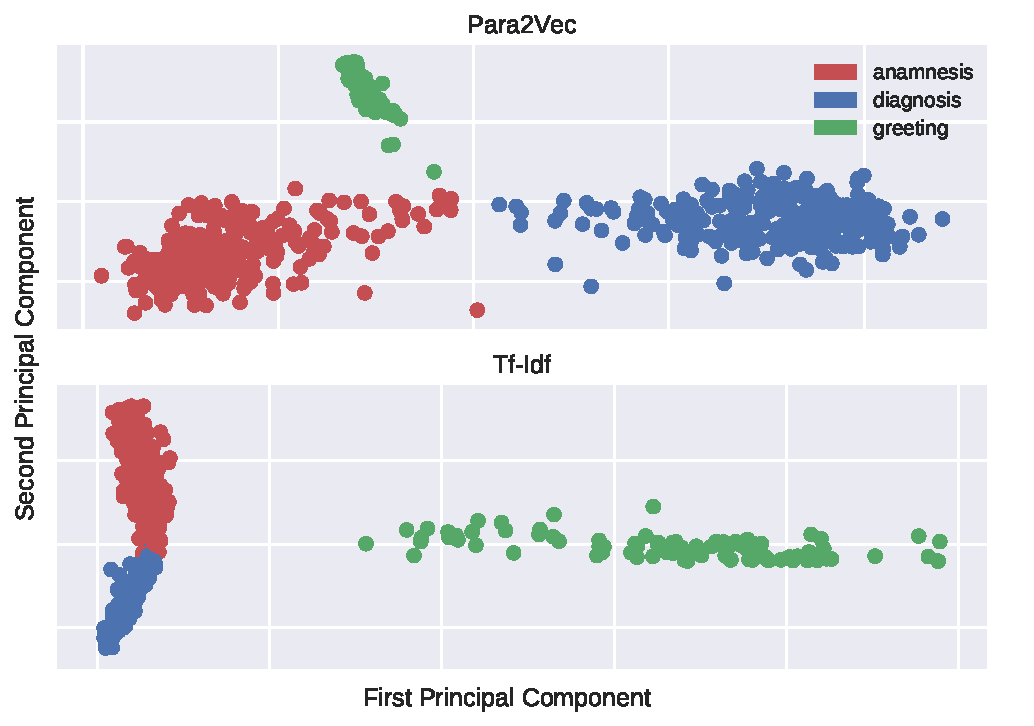
\includegraphics[width=\linewidth]{figures/para2vec_tfidf_pca}
	\caption{2D PCA projections of a vector space embedding of the physician letter paragraphs. Colors encode the respective paragraph category for each vector. \textbf{Top:} Paragraph vector space.  \textbf{Bottom:} Tf-idf vector space.}
	\label{fig:pv_tf_pca}
\end{figure}

\section{Disease Classification}
We tried to automatically assign to each letter which disease the patient had. This is useful for two reasons. First, people might want to search for all patients with a particular disease (more useful than full text search as diseases can be written many ways.) Second, many interesting pieces of information are not coded into a structured database, but are "hidden" in the free text. With these methods we can find this information.

\section{Letter Similarity}
With the vector embedding methods we are able to get an estimate of the dissimilarity of texts simply through a vector distance. This way we are able to suggest letters that are similar to a reference letter. As it worked better than expected we conducted the experiment detailed below


\end{document}